\begin{document}

\maketitle
\begin{frame}{Outline}
\setcounter{tocdepth}{1}
\tableofcontents
\end{frame}

\section{Religion and the Age of Reason}
\label{sec-1}
\begin{frame}[label=sec-1-1]{}
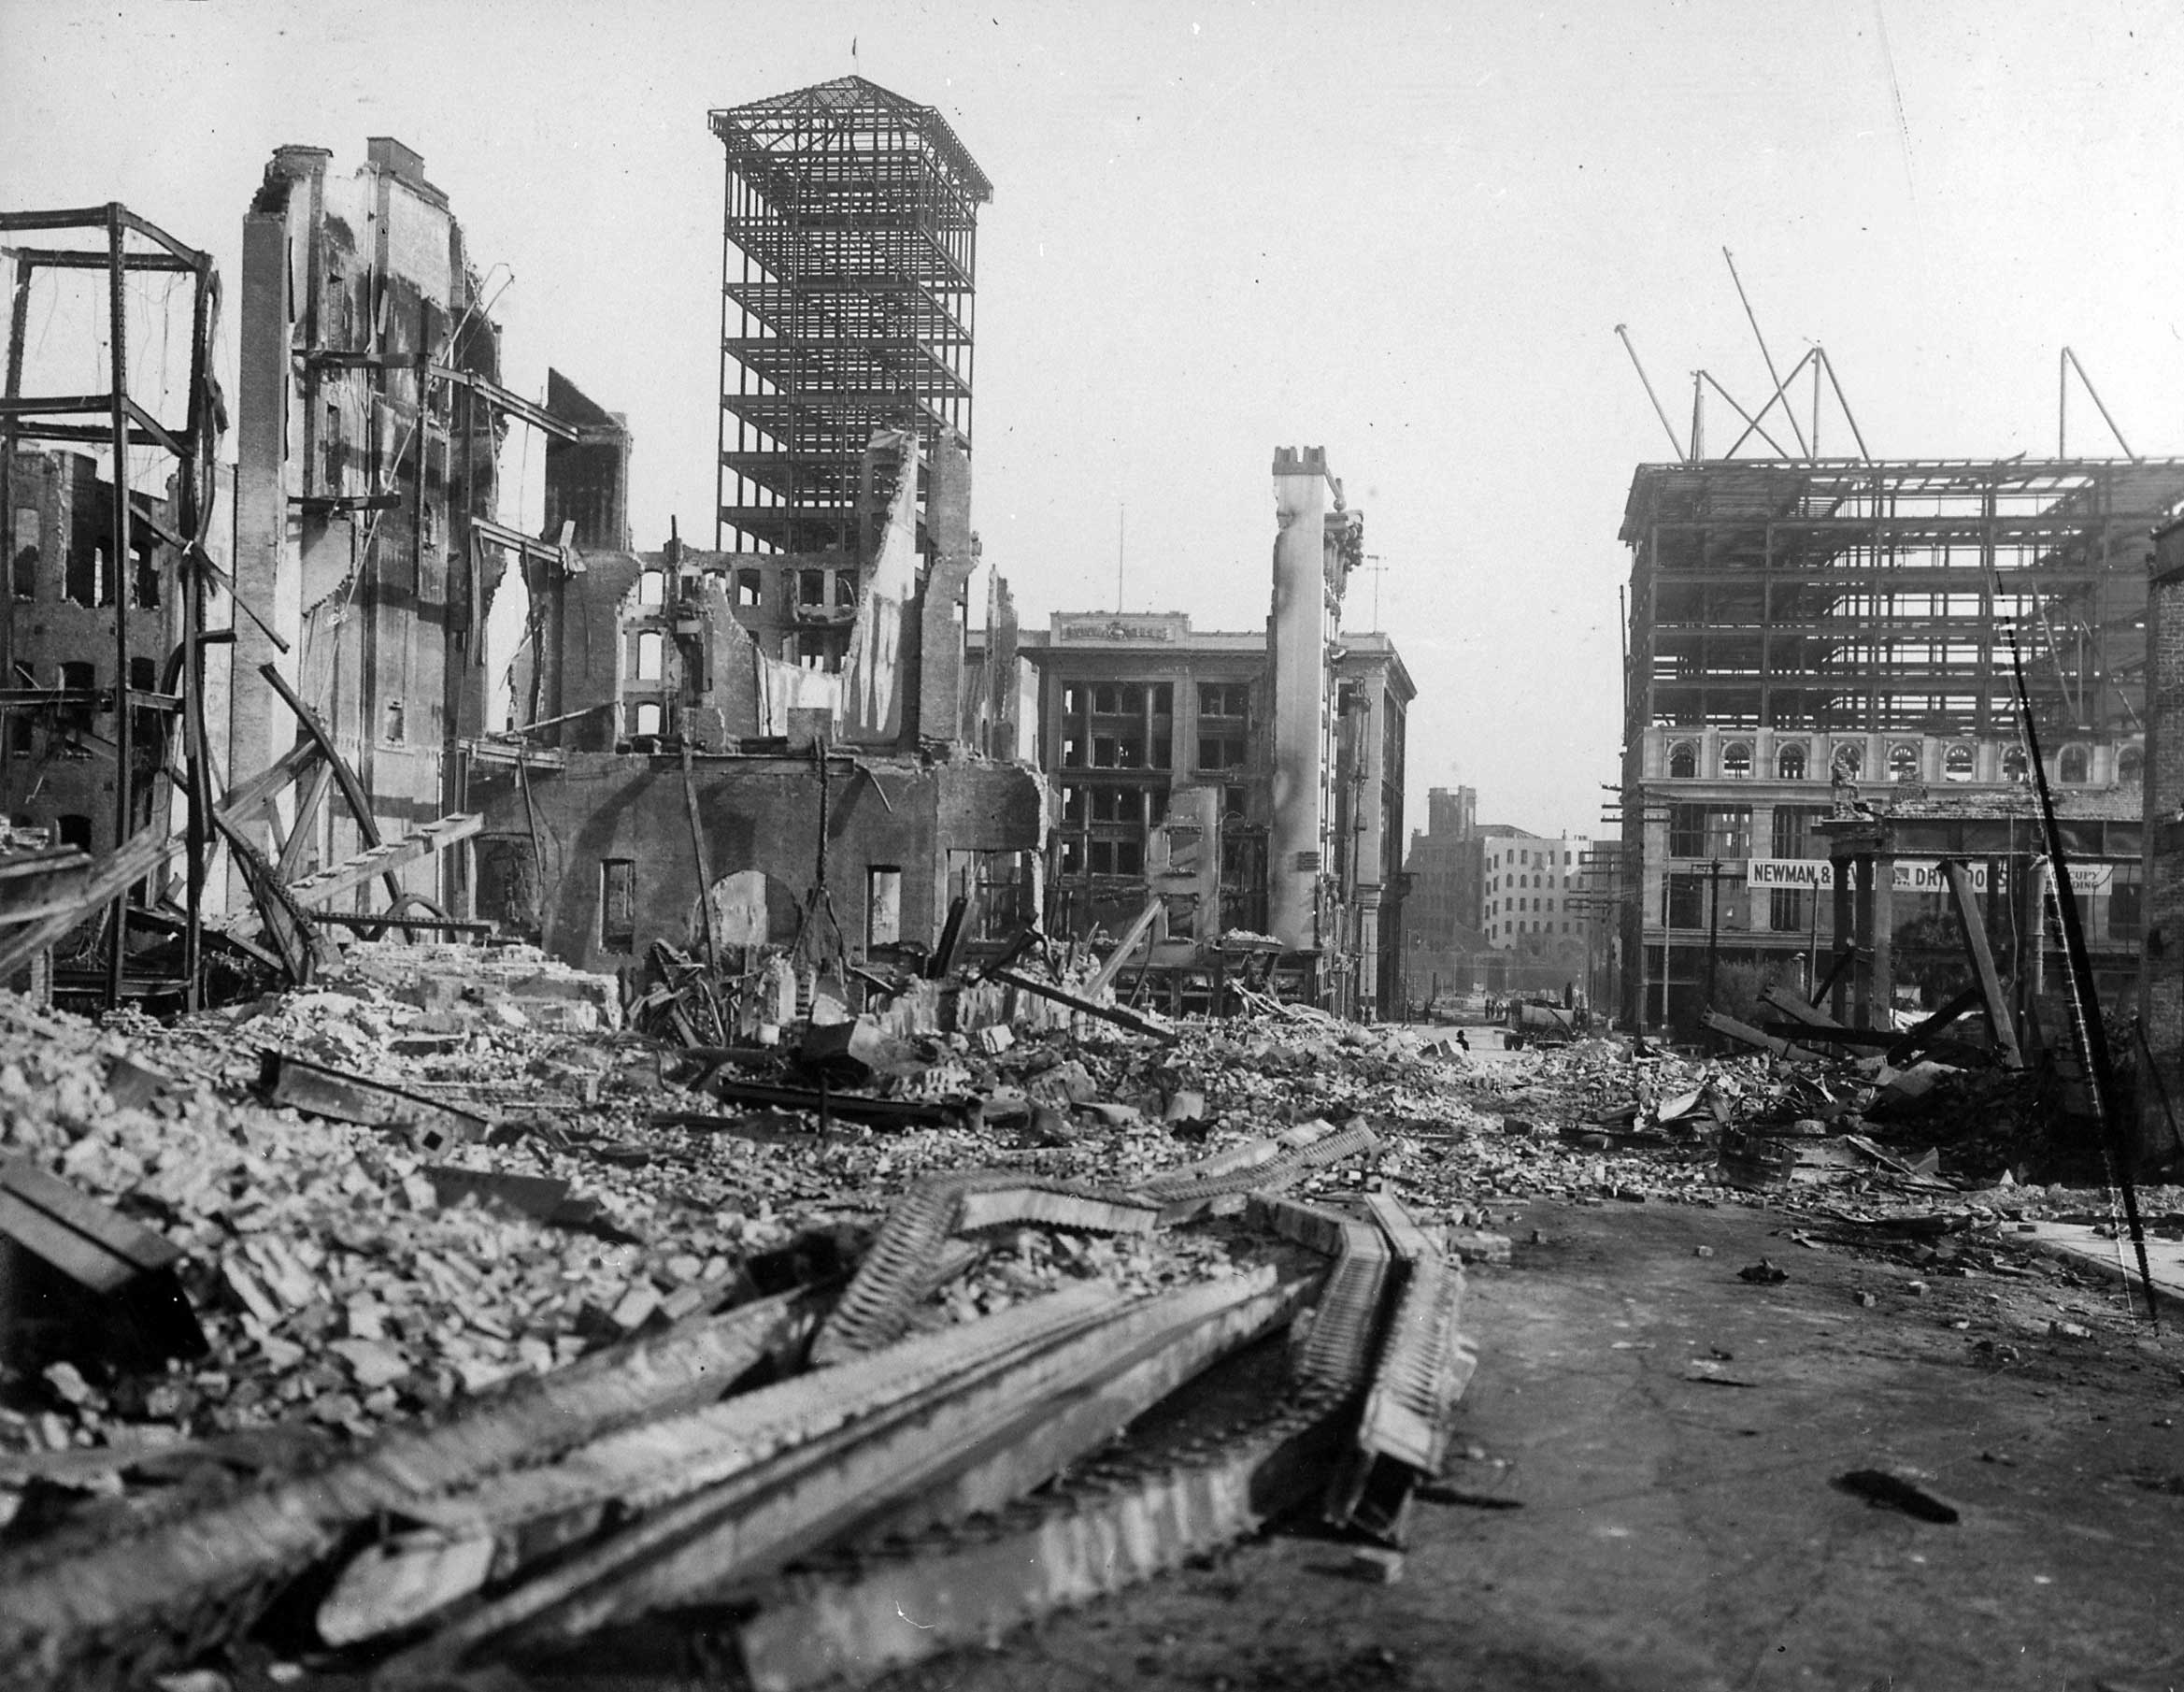
\includegraphics[width=.9\linewidth]{./img/sf-quakes.jpg}
\end{frame}

\begin{frame}[label=sec-1-2]{}
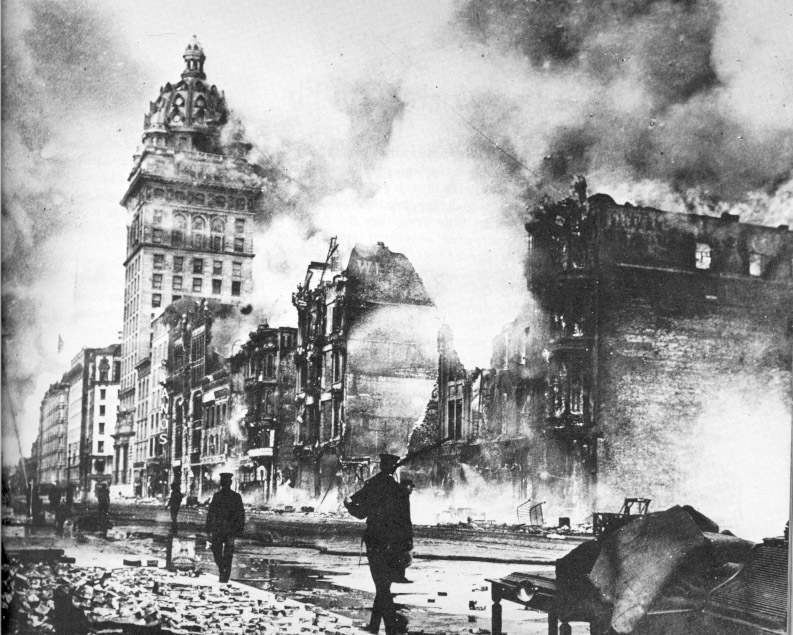
\includegraphics[width=.9\linewidth]{./img/sfeq06_01.jpg}
\end{frame}

\begin{frame}[label=sec-1-3]{}
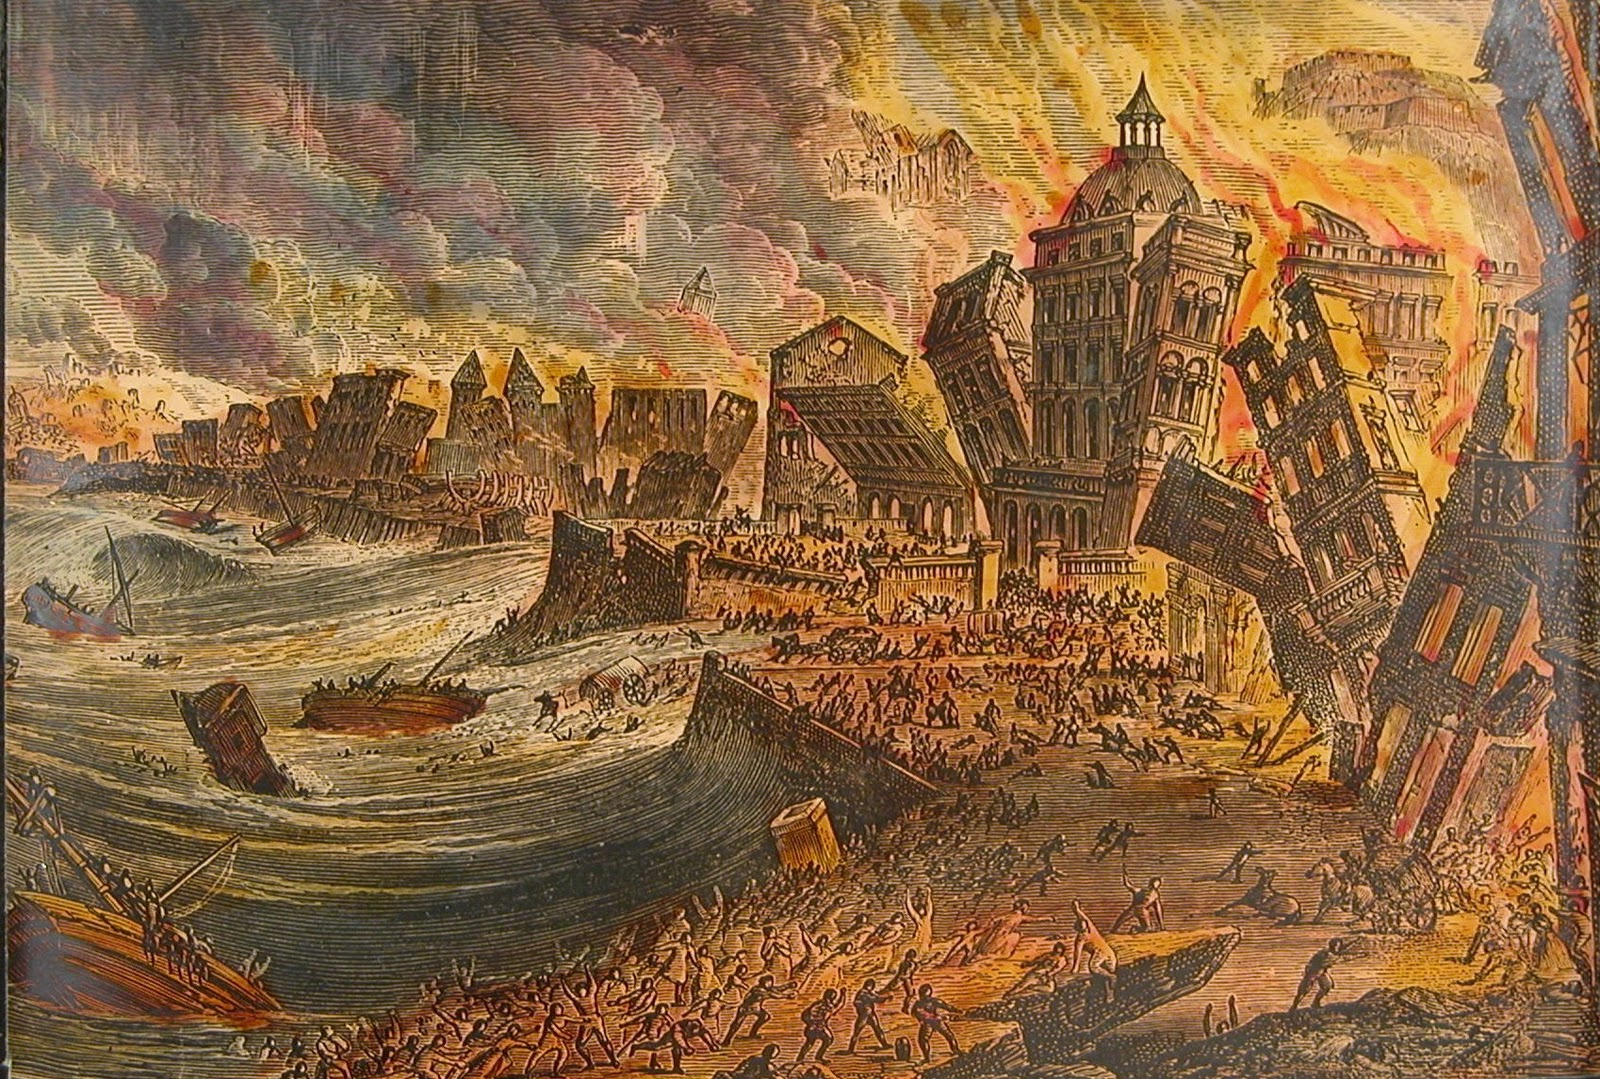
\includegraphics[width=.9\linewidth]{./img/lisbon-burning.jpeg}
\end{frame}

\begin{frame}[label=sec-1-4]{}
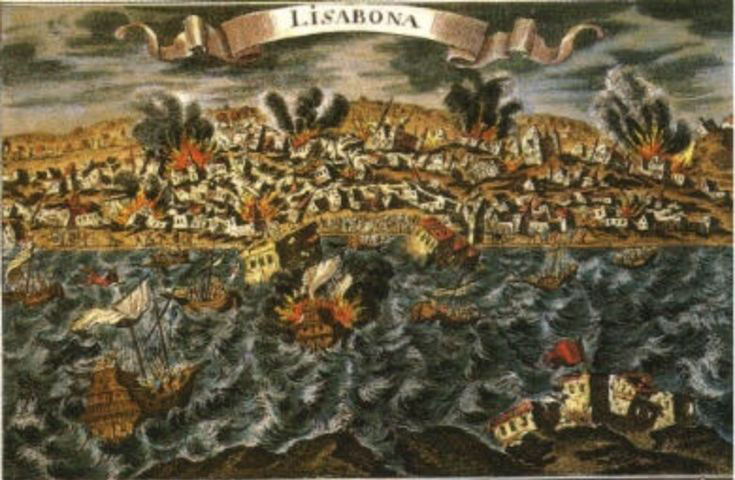
\includegraphics[width=.9\linewidth]{./img/Lisbon-earthquake-1755.jpg}
\end{frame}

\begin{frame}[label=sec-1-5]{Earthquakes and God's will}
\begin{itemize}
\item a tale of 2 earthquakes
\item he found the evidence for his belief in nature rather than in the Bible; he doubted a good bit of traditional doctrine—and he didn’t treat religion all that seriously.
\item Revivals but at heart a move from God to human beings
\end{itemize}
\end{frame}
\begin{frame}[label=sec-1-6]{From God-centered to Human-centered}
\begin{itemize}
\item 5 catalysts for change
\item at the very time of success in discovery and technology, reason seemed to reach its end of life
\item changing metaphor from Anselm to Descartes
\end{itemize}
\end{frame}

\begin{frame}[label=sec-1-7]{Religion of Reason}
\begin{itemize}
\item Cartesian coordinates
\item can a religion be built on Doubt?
\item No man shall ever be kept out of Heaven … if he had but an honest and good heart, that was ready to comply with Christ’s commandments
\item God is more inward to us than our very souls
\end{itemize}
\end{frame}

\begin{frame}[label=sec-1-8]{Descartes to Newton}
\begin{itemize}
\item Newton: God’s ``immensity'' stretching infinitely in all directions and unchanged for all eternity (cp. changing metaphor)
\item while retaining religion, it is no stripped of the ``supernatural''
\item Church of England would keep its theology vague enough to include as many groups as possible and tolerate the presence of some dissenting groups like Anabaptists and Quakers, though not Catholics
\end{itemize}
\end{frame}

\begin{frame}[label=sec-1-9]{Locke and Deists}
\begin{itemize}
\item Nearly all the attitudes of the time came together in John Locke
\item \url{https://www.youtube.com/watch?v=kItXvJLnTtk}
\item Many Deists brought to bear on the biblical miracle stories all the prestige of the scientific discovery of laws
\item Deists distrusted appeals to authority and the miraculous, but they also turned away from anything beyond natural religion in part for moral reasons.
\end{itemize}
\end{frame}
\begin{frame}[label=sec-1-10]{Pietists and Methodists}
\begin{itemize}
\item ``\alert{Enthusiasm}'' was a dirty word in the eighteenth century.
\item story begins in Germany, where Lutheran orthodoxy had increasingly defined faith as assent to a set of doctrines
\item Lutherans suspect any call to moral improvement as a move toward works-righteousness.
\item Methodism with a ``method'' for holiness
\item Wesley and Whitefield changed the shape of popular religion in England and North America, but they made little impact on the attitudes among most intellectuals
\end{itemize}
\end{frame}
\begin{frame}[label=sec-1-11]{The end of Reason}
\begin{itemize}
\item Hume
\item Rousseau
\item Kant
\end{itemize}
\end{frame}
% Emacs 24.3.1 (Org mode 8.2.3c)
\end{document}
